\chapter{Integration: Adding Countless Small Quantities}

\section{An Odometer Accumulates Distance}

Sit in a car and look at two instruments: the speedometer shows how fast you are moving now, and the odometer shows how far you have travelled altogether. Last chapter asked how a changing odometer reading determines velocity at each instant. The answer was differentiation: divide the distance increase over a short interval by that interval, then let the interval shrink toward zero.

Now reverse the question. Suppose the odometer is broken but the speedometer works, recording the current speed every second. Can those records alone tell you the total distance travelled?

Intuition suggests this: during the first second, speed is about $20$ metres per second, so distance is about $20$ metres; during the second, speed is about $22$ metres per second, so distance is about $22$ metres. Add these distances for an approximate total. Record every tenth of a second instead, and speed changes less within each interval, so the sum should be more accurate.

Such instrument pairs are everywhere. A tap's flow is a rate; the water meter records an amount. Electrical power is a rate; the electricity meter records energy. Network speed is a rate; a phone's data-usage counter records an amount. Every total-amount meter quietly accumulates an instantaneous rate continuously. This chapter asks exactly what operation that accumulation is.

The simplest idea---\emph{divide a process into many small intervals, treat each as approximately uniform, and add all their contributions}---is the starting point of integration. The same idea finds areas bounded by curves, volumes of spheres and cones, work done by varying forces, and probabilities of random events. It also answers a remarkable question: when can adding infinitely many numbers produce a finite answer?

\section{A Problem That Stalled Mathematics for Two Thousand Years}

Begin with a more geometrical question. The parabola $y=1-x^{2}$ and the $x$-axis enclose a little hill, with $x$ from $-1$ to $1$. What is its area?

You can calculate triangles and rectangles, and you have memorized a circle's area formula. But this hill has a curved boundary and is neither polygon nor circle. Guess intuitively: its enclosing rectangle has width $2$, height $1$, and area $2$. Its largest inscribed triangle has base $2$, height $1$, and area $1$. So the answer lies between $1$ and $2$. Can you narrow it? Some guess $1.5$, others near $1.3$. Intuition alone has run out.

Ancient mathematicians had impressive successes with curved boundaries. To find a circle's area, Liu Hui in China's Wei--Jin period used polygonal exhaustion: inscribe a regular hexagon, then a dodecagon, then a twenty-four-sided polygon, and keep doubling. Each polygon fits the circle more closely. He explained that finer cutting loses less, and repeated cutting ultimately coincides with the circumference without loss. This is a mature idea of limits, more than a thousand years before comparable European approaches.

Archimedes in ancient Greece tackled the parabolic hill. He filled it with successive layers of shrinking triangles: one large triangle, then two smaller ones, then four smaller still. He proved that each layer's total area is exactly one quarter of the preceding layer, giving
\[
S=1+\frac14+\frac1{16}+\frac1{64}+\cdots
\]
He also proved that the infinite sum is $\dfrac43$. Thus the parabolic region has exactly $\dfrac43$ times the area of its large inscribed triangle. Without algebraic notation or coordinates, this was a feat like climbing a cliff barehanded.

Yet Archimedes' method has an unsettling feature: every new curve demands a newly invented cutting technique, like forging a separate key for every lock. Circles need one method, parabolas another, spirals another, each relying on a construction visible only to genius. Could there be a \emph{master key}, one routine for every curve? The question stalled mathematicians for nearly two thousand years.

\section{First Attempt: Too Few Rectangles, Too Much Error}

The natural attempt uses rectangles. Divide $[-1,1]$ into intervals, erect a rectangle on each with a height taken from the curve, and add their areas to approximate the hill.

Try two intervals. On each half, height varies from $0$ to $1$. Using the maximum height $1$ gives rectangles of area $1\times 1=1$ each and total $2$, the enclosing rectangle, visibly too large at the corners. Using the minimum gives height $0$ at the left endpoint and $0$ at the right endpoint, for total $0$, absurdly small. The true area lies between $2$ and $0$, but the gap is too large to tell us much.

Four intervals improve matters, ten improve them further, and a hundred further still. A reassuring rule appears: the upper sum using maxima is never below the true area; the lower sum using minima is never above it. Doubling the divisions pushes the upper sum down and the lower sum up, squeezing their gap. The true area is like a prisoner between approaching walls. Yet finitely many flat-topped rectangles leave a gap against a curved boundary. We cannot call $100$ rectangles the answer, only say that $100$ rectangles give an approximation near it. What is the answer itself? Must we forever approach without arriving?

\begin{fanli}
``More rectangles give greater accuracy, so a million rectangles give the exact value.'' This sounds plausible but confuses concepts. A million is still finite, the tops are still flat, and the result remains an approximation with a small error. Excellent approximation and exact equality differ. Integration's crucial step goes beyond every finite subdivision: let the number of pieces grow without bound and take the \emph{limit} of the approximations. Recall Chapter 9: the limit is the exact destination.
\end{fanli}

\section{Turning Finer Subdivision into a Definition}

The way out is to recognize that we need a limiting process, not a larger finite number. Divide $[a,b]$ into $n$ intervals, each of width $\Delta x=\dfrac{b-a}{n}$. Choose any point in interval $i$ and record the curve's height $f(x_i)$. Its rectangle contributes approximately $f(x_i)\,\Delta x$. Add them:
\[
S_n=f(x_1)\,\Delta x+f(x_2)\,\Delta x+\cdots+f(x_n)\,\Delta x .
\]
This is a \emph{Riemann sum}. As $n$ grows and $\Delta x$ shrinks, suppose $S_n$ approaches a definite $S$, independent of the sample points chosen. Then $f$ is integrable on $[a,b]$, and $S$ is its definite integral.

\begin{dingyi}[Definite Integral]
Let $f$ be defined on $[a,b]$. Divide $[a,b]$ into $n$ equal intervals of width $\Delta x=\dfrac{b-a}{n}$, and choose a point $x_i$ in each. If, as $n\to\infty$, the Riemann sum
\[
S_n=\sum_{i=1}^{n} f(x_i)\,\Delta x
\]
has a limit independent of the chosen points, that limit is the \emph{definite integral} of $f$ on $[a,b]$, written
\[
\int_a^b f(x)\,dx=\lim_{n\to\infty}\sum_{i=1}^{n} f(x_i)\,\Delta x .
\]
\end{dingyi}

\begin{zhu}
Not every imaginable function is integrable. Fortunately, the functions encountered here, including continuous functions and those with only a few jump discontinuities, are integrable. Investigating the full boundary of integrability belongs to university real analysis. Independence from sample points matters: if changing the points changes the limit, the function is too wild to yield a definite area this way.
\end{zhu}

\begin{center}
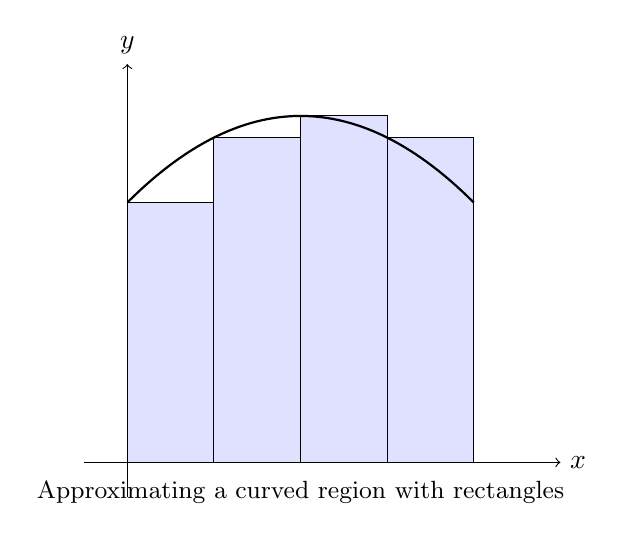
\begin{tikzpicture}[scale=1.1]
  \draw[->] (-0.5,0) -- (5,0) node[right] {$x$};
  \draw[->] (0,-0.4) -- (0,4.6) node[above] {$y$};
  \draw[fill=blue!12] (0,0) rectangle (1,3);
  \draw[fill=blue!12] (1,0) rectangle (2,3.75);
  \draw[fill=blue!12] (2,0) rectangle (3,4);
  \draw[fill=blue!12] (3,0) rectangle (4,3.75);
  \draw[thick,domain=0:4,samples=60] plot (\x,{4-0.25*(\x-2)*(\x-2)});
  \node at (2,-0.35) {\small Approximating a curved region with rectangles};
\end{tikzpicture}
\end{center}

What does $\int$ accomplish? It compresses the entire limiting process of cutting into infinitely many tiny pieces and adding them into one symbol. This elongated S, for sum, reminds us that integration is addition carried to a limit. The expression $f(x)\,dx$ resembles an infinitesimal rectangle's area, with height $f(x)$ and width $dx$.

\begin{shuyu}{Definite Integral}
\textbf{Intuition:} the exact area of a curved region, approached by sums of increasingly narrow rectangles.

\textbf{Formal definition:} the limit of Riemann sums as the subdivision becomes arbitrarily fine, written $\int_a^b f(x)\,dx$.

\textbf{Example:} $\int_0^2 x\,dx=2$, exactly the area of a triangle with base $2$ and height $2$.
\end{shuyu}

Return to the odometer. Divide the journey into $n$ short intervals. In interval $i$, approximate velocity by $v(t_i)$ and distance by $v(t_i)\,\Delta t$, making the total a Riemann sum. Let $n\to\infty$ to get
\[
\text{total distance}=\int_a^b v(t)\,dt .
\]
On a velocity-time graph, $v(t_i)\,\Delta t$ is a thin rectangle's area, so \emph{distance is the area under the velocity curve}. Integration connects a rate with an amount. At constant speed, the graph is horizontal and its area a rectangle, recovering the primary-school rule of distance equals speed times time. Integration extends that rule to arbitrary variation in speed.

\section{The Master Key: The Fundamental Theorem of Calculus}

We have a definition, but calculating every integral by a Riemann-sum limit would be little better than forging a new key each time. Calculus offers a magnificent gift: to calculate a definite integral, find a function whose derivative is $f$, and no direct limit calculation is needed.

\begin{dingli}[The Fundamental Theorem of Calculus]
Let $f$ be continuous on $[a,b]$, and let $F$ be an antiderivative of $f$, meaning $F'(x)=f(x)$. Then
\[
\int_a^b f(x)\,dx=F(b)-F(a).
\]
\end{dingli}

Why is this true? Distance and velocity make it clearest. If $s(t)$ is the odometer reading, then $v(t)=s'(t)$ by the definition of derivative. Between times $a$ and $b$, the total odometer increase is $s(b)-s(a)$. But our integral calculation says the same distance is $\int_a^b v(t)\,dt$. Therefore
\[
\int_a^b v(t)\,dt=s(b)-s(a).
\]
Replace $v$ by $f$ and $s$ by $F$, and this is the theorem. Let us make the intuition more like a proof.

\begin{proof}
Divide $[a,b]$ into $n$ equal intervals with endpoints $a=t_0<t_1<\cdots<t_n=b$ and width $\Delta t$. The total increment is a sum of smaller increments:
\[
F(b)-F(a)=\bigl[F(t_1)-F(t_0)\bigr]+\bigl[F(t_2)-F(t_1)\bigr]+\cdots+\bigl[F(t_n)-F(t_{n-1})\bigr],
\]
where the middle terms cancel in pairs, leaving the endpoints. By the meaning of derivative, for small $\Delta t$ each interval satisfies
\[
F(t_i)-F(t_{i-1})\approx F'(t_{i-1})\,\Delta t=f(t_{i-1})\,\Delta t ,
\]
so $F(b)-F(a)$ approximates the Riemann sum $\sum f(t_{i-1})\,\Delta t$. Let $n\to\infty$: approximation becomes an exact limit. The left side $F(b)-F(a)$ is independent of subdivision, while the right tends to $\int_a^b f(t)\,dt$, so they are equal.
\end{proof}

The crucial step is the cancellation of the long chain of intermediate terms, leaving $F(b)-F(a)$. Through that cancellation, integration's total accumulation fits exactly with differentiation's local rate of change. This is why \emph{differentiation and integration are inverse operations}.

\begin{zhu}
Antiderivatives are not unique: $x^{2}$ has derivative $2x$, and $x^{2}+7$ also has derivative $2x$, since a constant disappears under differentiation. This does not affect the theorem. Two antiderivatives differ by a constant, which cancels in $F(b)-F(a)$. Choose whichever antiderivative is most convenient.
\end{zhu}

Try a numerical example. For the parabolic hill, calculate $\int_{-1}^{1}(1-x^{2})\,dx$. Which function differentiates to $1-x^{2}$? Try $F(x)=x-\dfrac{x^{3}}{3}$; indeed, $F'(x)=1-x^{2}$. Thus
\[
\int_{-1}^{1}(1-x^{2})\,dx=F(1)-F(-1)=\left(1-\frac13\right)-\left(-1+\frac13\right)=\frac43 .
\]
$\dfrac43$! Exactly Archimedes' answer from infinitely many triangles. Two thousand years later, the master key agrees with the old locksmith, one of mathematics' most reassuring moments.

\begin{toolbox}
This chapter's new tools:
\begin{itemize}
  \item \textbf{Riemann sums}: divide intervals finely and approximate curved areas with rectangle sums.
  \item \textbf{Definite integral} $\int_a^b f(x)\,dx$: a limit of Riemann sums, geometrically the area under a curve.
  \item \textbf{The fundamental theorem of calculus}: find an antiderivative $F$, then the integral is $F(b)-F(a)$. Differentiation and integration undo each other.
  \item \textbf{Slicing}: volume is the integral of cross-sectional area; solids with equal cross-sections at every height have equal volumes.
  \item \textbf{Series tests, intuitively}: terms tending to $0$ are necessary but insufficient for convergence. Geometric series converge when the common ratio's absolute value is below $1$.
\end{itemize}
\end{toolbox}

\begin{lianjie}
This theorem sews three chapters together: Chapter 9's limits give the integral's definition, Chapter 10's derivatives supply its calculation key, and integration reconstructs total amounts from rates. Chapter 12 will show how scrutinizing conditions such as continuity and existence of limits gave rise to rigorous analysis.
\end{lianjie}

\section{Slicing Bread: From Area to Volume}

Integration does more than area. How do we find a cone's or sphere's volume? Middle-school formulas say that a cone has one third the volume of a cylinder with the same base and height, and a sphere has volume $\dfrac{4}{3}\pi r^{3}$. Then we could only memorize them; now we can ask why.

Use the same method: cut. Imagine a sphere as a loaf sliced perpendicular to a horizontal axis. At position $x$ from the centre, with the centre at $0$ and ends at $-r$ and $r$, the section is a circle. Pythagoras gives squared radius $r^{2}-x^{2}$ and area $\pi\left(r^{2}-x^{2}\right)$. A slice of thickness $\Delta x$ has approximate volume $\pi\left(r^{2}-x^{2}\right)\Delta x$. Add and take the limit:
\[
V=\int_{-r}^{r}\pi\left(r^{2}-x^{2}\right)dx .
\]
The integrand is only quadratic, so an antiderivative is easy: $F(x)=\pi\left(r^{2}x-\dfrac{x^{3}}{3}\right)$. The fundamental theorem gives
\[
V=F(r)-F(-r)=\pi\left(r^{3}-\frac{r^{3}}{3}\right)-\pi\left(-r^{3}+\frac{r^{3}}{3}\right)=\frac{4}{3}\pi r^{3} .
\]
The formula once memorized is the result of one integral.

Legend says Archimedes was proudest of the relation between a sphere and its enclosing cylinder, of base radius $r$ and height $2r$: the sphere has two thirds its volume. He requested the figure on his tomb. Without integral notation, he compared slices: at each height, the sphere's section plus a cone's section equals the cylinder's section. In ancient China, Zu Geng, son of Zu Chongzhi, summarized the same idea: equal cross-sectional areas at every equal height force equal volumes. The principle later became known in Europe under Cavalieri's name, more than a thousand years after Zu Geng. Its independent growth in two civilizations suggests how naturally slicing approaches volume.

The cone's one-third factor follows similarly. Stand a cone of height $h$ and base radius $r$ with its tip upward. At distance $x$ below the vertex, similar triangles give section radius $\dfrac{rx}{h}$ and area $\pi\dfrac{r^{2}x^{2}}{h^{2}}$. Thus
\[
V=\int_0^{h}\pi\frac{r^{2}x^{2}}{h^{2}}\,dx=\frac{\pi r^{2}}{h^{2}}\cdot\frac{h^{3}}{3}=\frac13\pi r^{2}h .
\]
Pull the constant $\dfrac{\pi r^{2}}{h^{2}}$ outside, leaving the familiar $\int_0^{h}x^{2}dx=\dfrac{h^{3}}{3}$. Volume formulas become consequences of one statement: volume is the integral of cross-sectional area.

\section{Another Perspective: Density, Probability, and Soup}

Wherever a rate accumulates into an amount, integration appears. Consider three examples beyond area and volume.

\textbf{Mass and density.} An uneven metal rod is less dense at the left and denser at the right. Its linear density at position $x$ is $\rho(x)$, mass per unit length. Divide it into $n$ pieces. Piece $i$ is approximately uniform, with mass $\rho(x_i)\,\Delta x$. Summing and taking the limit gives
\[
\text{total mass}=\int_a^b \rho(x)\,dx .
\]
In a pot of soup with uneven salt concentration, total salt is likewise the integral of concentration over volume, a three-dimensional integral studied at university.

\textbf{Electricity and work.} Current is the rate of charge flow, so total charge over an interval is the integral of current over time. If current rises as $I(t)=2t$ amperes, charge flowing in the first three seconds is
\[
\int_0^3 2t\,dt=3^{2}-0^{2}=9\ \text{coulombs} .
\]
Similarly, work over a displacement is the integral of force with respect to displacement. A spring becomes harder to stretch as its extension grows; integration calculates the total work of that changing force.

\textbf{Probability and density.} You wait at a station, with the bus equally likely to arrive at any time during one hour. What is the probability of arrival between $10$ o'clock and $10$:$15$? Intuition gives $\dfrac14$, since the interval occupies a quarter of the hour. But if arrivals are more frequent toward evening, their likelihood varies with time. A \emph{density curve} $p(x)$ describes the probability concentration per unit time near $x$. Then
\[
P(\text{arrival between }c\text{ and }d\text{ })=\int_c^d p(x)\,dx ,
\]
so probability is area under the density curve. Total probability is $1$, meaning that the integral over the full range is $1$. In our uniform example the density is $\dfrac{1}{60}$ per minute, a horizontal line, and probability is rectangle area. Densities for random quantities such as height and measurement error are bell-shaped, high in the middle and low at both ends; Chapter 18 studies them.

\begin{shuyu}{Probability Density}
\textbf{Intuition:} a curve whose area over an interval gives the probability that a random quantity falls in that interval.

\textbf{Formal definition:} a nonnegative function $p(x)$ whose integral over the entire range equals $1$, with $P(c\le X\le d)=\int_c^d p(x)\,dx$.

\textbf{Example:} $p(x)=\dfrac1{60}$ for $0\le x\le 60$ minutes describes uniform arrival over an hour. The probability of arriving within a quarter-hour is $\dfrac{15}{60}=\dfrac14$.
\end{shuyu}

A counterintuitive feature matters: a density curve's height at one point is not a probability. Arriving exactly at $10$:$30$:$00$ has probability $0$, since a single point has zero interval width and zero area. Probability belongs to intervals; density describes concentration. This is the same distinction as velocity at an instant versus distance. Integration accumulates a rate into an amount.

\section{When Does Infinite Addition Give a Finite Result?}

Archimedes' area calculation contains another treasure: $1+\dfrac14+\dfrac1{16}+\cdots=\dfrac43$. Infinitely many positive numbers produce a finite total. Intuition protests: should infinitely many things not add to infinity?

Not necessarily. Chapter 9's Zeno discussion already planted the answer. To travel $1$ kilometre, first travel $\dfrac12$, then $\dfrac14$, then $\dfrac18$, and continue. Infinitely many stages still give a finite distance:
\[
\frac12+\frac14+\frac18+\cdots=1.
\]
Geometry makes this clearer. Colour half a unit square, then half the remainder, then half again. Each step approaches complete coverage while leaving a little uncoloured. The total coloured area tends to $1$ without exceeding it.

\begin{center}
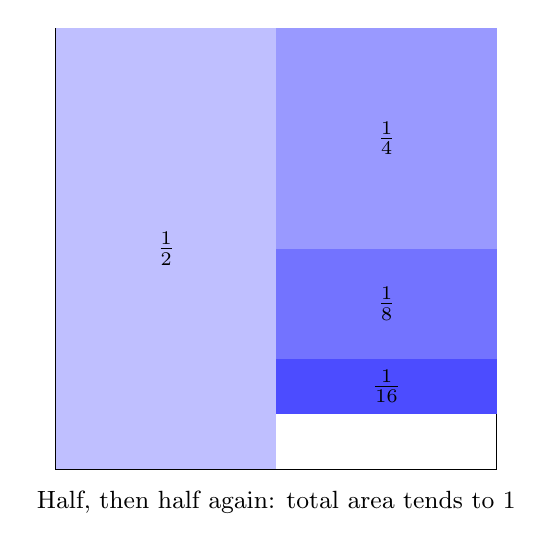
\begin{tikzpicture}[scale=1.4]
  \draw (0,0) rectangle (4,4);
  \fill[blue!25] (0,0) rectangle (2,4);
  \fill[blue!40] (2,2) rectangle (4,4);
  \fill[blue!55] (2,1) rectangle (4,2);
  \fill[blue!70] (2,0.5) rectangle (4,1);
  \node at (1,2) {$\frac12$};
  \node at (3,3) {$\frac14$};
  \node at (3,1.5) {$\frac18$};
  \node at (3,0.75) {$\frac1{16}$};
  \node at (2,-0.3) {\small Half, then half again: total area tends to $1$};
\end{tikzpicture}
\end{center}

A sum with the same ratio between successive terms is a \emph{geometric series}. If its ratio $q$ satisfies $|q|<1$, it has a finite sum:
\[
a+aq+aq^{2}+\cdots=\frac{a}{1-q}.
\]
For Zeno's example, $a=\dfrac12$ and $q=\dfrac12$, giving $\dfrac{1/2}{1-1/2}=1$. The proof is simple: set $S=a+aq+\cdots+aq^{n}$ and multiply by $q$ to get $qS=aq+\cdots+aq^{n+1}$. Subtract and cancel the middle terms: $(1-q)S=a-aq^{n+1}$. When $|q|<1$ and $n\to\infty$, $q^{n+1}\to 0$, so $S\to\dfrac{a}{1-q}$. Again \emph{cancellation} leads the way, echoing the fundamental theorem's proof.

Repeating decimals hide geometric series too. Does $0.999\ldots$ equal $1$? Expand it:
\[
0.999\ldots=0.9+0.09+0.009+\cdots=\frac{0.9}{1-0.1}=1 .
\]
It \emph{is} $1$, rather than merely approaching $1$, wearing an infinitely long disguise. The limit itself is the destination, not the unfinished process.

Some series converge extremely quickly. A famous example appears in the natural logarithm's base $e$:
\[
e=1+1+\frac12+\frac16+\frac1{24}+\frac1{120}+\cdots
\]
The denominators are successive products: $2=1\times2$, $6=1\times2\times3$, $24=1\times2\times3\times4$, and so on. Each denominator gains another growing factor, making terms shrink faster than any geometric series. The first seven terms give $e\approx2.718$, accurate to two decimal places. Compound interest, population growth, and radioactive decay all involve this number, whose face turns out to be a rapidly converging infinite sum. Next chapter's power-series expansions return to it.

But do not infer that shrinking terms guarantee a finite sum. The best-known counterexample is the \emph{harmonic series}:
\[
1+\frac12+\frac13+\frac14+\frac15+\cdots
\]
Its terms tend to $0$, yet its sum is infinite.

\begin{dingli}[The Harmonic Series Diverges]
The sum of $1+\dfrac12+\dfrac13+\dfrac14+\cdots$ exceeds every prescribed number.
\end{dingli}

\begin{proof}
Group the terms: first $1$, then $\dfrac12$, then $\dfrac13+\dfrac14$. Each term in that third group is at least $\dfrac14$, so its sum exceeds $\dfrac14+\dfrac14=\dfrac12$. The fourth group, $\dfrac15+\dfrac16+\dfrac17+\dfrac18$, has four terms each at least $\dfrac18$, so it exceeds $4\times\dfrac18=\dfrac12$. The next $8$ terms are each at least $\dfrac1{16}$ and again total more than $\dfrac12$. Each doubling of the term count supplies at least another $\dfrac12$. Adding $\dfrac12$ infinitely often exceeds every bound.
\end{proof}

This proof, first given by a medieval scholar, is surprisingly simple but profound. Terms tending to $0$ are a \emph{necessary condition} for convergence, far from sufficient. Convergence depends on shrinking quickly enough. The sum of all $\dfrac1{n^{2}}$ converges, in fact to $\dfrac{\pi^{2}}{6}$: pi emerges from a collection of squares! Euler discovered this as a young man, astonishing the mathematical world. The sum of all $\dfrac1n$ diverges. What about $\dfrac1{n^{1.5}}$ or $\dfrac1{n^{1.001}}$? Locating the boundary between fast and slow is one of analysis's most delicate questions.

\begin{fanli}
``The terms tend to $0$, so the sum is finite.'' The harmonic series refutes this directly. The reverse implication does hold: a finite sum forces terms to tend to $0$, but terms tending to $0$ do not imply a finite sum. Necessary and sufficient conditions differ by more than a word.
\end{fanli}

\section{Approximating an Integral by Hand}

\begin{shiyan}
Take squared paper and check the fundamental theorem yourself.

\begin{enumerate}
  \item Plot $y=x^{2}$ on $0\le x\le 2$. Divide $[0,2]$ into $4$ intervals of width $0.5$, erect rectangles using \emph{right-endpoint} heights, and add their areas:
  \[
  0.5\times(0.5^{2}+1^{2}+1.5^{2}+2^{2})=0.5\times 7.5=3.75 .
  \]
  Repeat with \emph{left-endpoint} heights: $0.5\times(0+0.25+1+2.25)=1.75$. The true area lies between these values.
  \item Find the exact value using the fundamental theorem. An antiderivative of $x^{2}$ is $\dfrac{x^{3}}{3}$, so
  \[
  \int_0^2 x^{2}\,dx=\frac{2^{3}}{3}-0=\frac83\approx 2.67 .
  \]
  It does lie between $1.75$ and $3.75$.
  \item Increase to $8$ intervals of width $0.25$. Recalculate both rectangle sums, record them below, and observe how they squeeze toward $\dfrac83$:
\end{enumerate}
\begin{center}
\begin{tabular}{cccc}
\toprule
Intervals $n$ & Left-endpoint sum & Right-endpoint sum & Exact value $\frac83$ \\
\midrule
$4$ & $1.75$ & $3.75$ & $2.666\ldots$ \\
$8$ & $2.19$ & $3.19$ & $2.666\ldots$ \\
\bottomrule
\end{tabular}
\end{center}
If you wish, calculate $n=16$ with a calculator. How much does each approximation improve? Guess the rate at which the error shrinks.
\end{shiyan}

\begin{pandeng}
Further signposts include \emph{integration by substitution} and \emph{integration by parts}, two tools for calculating integrals; \emph{improper integrals}, handling infinite intervals or unbounded integrands, such as $\int_1^{\infty}\frac{1}{x^{2}}dx=1$; \emph{numerical integration}, using trapezoids or parabolas for efficient computation; the \emph{Riemann $\zeta$ function}, where the convergence boundary of $\sum\frac{1}{n^{s}}$ leads to Chapter 15's primes; and the more general \emph{Lebesgue integral}, which replaces vertical strips with horizontal layers to handle stranger functions.
\end{pandeng}

\section*{Questions to Think About}

\textbf{Observation}
\begin{sikao}
  \item A speedometer always shows a positive reading, but the driver goes forward and then reverses to the start. Are the area under the velocity curve and total distance still the same? Hint: should reverse motion be recorded as positive or negative velocity? What do the integral and the actual distance wearing down the odometer each represent?
  \item Examine a water meter, electricity meter, and phone data-usage counter. Does each record a rate or an amount? What is its partner quantity? Hint: each rate-amount pair hides an integral and a derivative.
\end{sikao}

\textbf{Proof}
\begin{sikao}
  \item Without consulting a formula, prove $\dfrac13+\dfrac19+\dfrac1{27}+\cdots=\dfrac12$. Hint: multiply by $q$ and subtract as in the text, or draw a square and repeatedly take thirds.
  \item Use the fundamental theorem to explain why $\int_a^b x\,dx=\dfrac{b^{2}-a^{2}}{2}$ equals the area of a trapezoid. Hint: what figure does $y=x$ enclose over $[a,b]$, and how long are the two parallel sides?
\end{sikao}

\textbf{Challenge}
\begin{sikao}
  \item The harmonic series diverges, but deleting all terms whose denominators contain the digit $9$, such as $\dfrac19$, $\dfrac1{19}$, and $\dfrac1{92}$, leaves a convergent sum. Can you estimate why? Hint: how many one-digit, two-digit, and three-digit numbers omit $9$? What bounds the sum of their reciprocals in each group? Try summing those bounds geometrically.
  \item The proof of $\int_a^b f(x)\,dx=F(b)-F(a)$ assumes that $F$ has derivative $f$. If we know only that $f$ is continuous, can we \emph{construct} an antiderivative? Hint: consider $F(x)=\int_a^x f(t)\,dt$ and estimate $\dfrac{F(x+h)-F(x)}{h}$ for small $h$. Next chapter makes this idea rigorous.
\end{sikao}

\section*{The Door to the Next Chapter}

We have moved quickly enough that our footing may feel uncertain. What does existence of a Riemann-sum limit mean? Why must approaching upper and lower sums squeeze out exactly one number rather than leave a permanent gap? The fundamental theorem requires $f$ to be continuous, but can drawing without lifting a pencil be a definition? Behind the divergence of the harmonic series and convergence of $\sum\frac{1}{n^{2}}$, is there one common measuring tool?

These questions are easy to understand and beautifully difficult to answer. Nineteenth-century mathematicians forged everyday words such as approach, continuity, and convergence into precise definitions, creating \emph{analysis}. Next chapter we enter that workshop to see intuition forged into theorems, and meet an old friend there: constructing any complicated sound from infinitely many simple waves.
